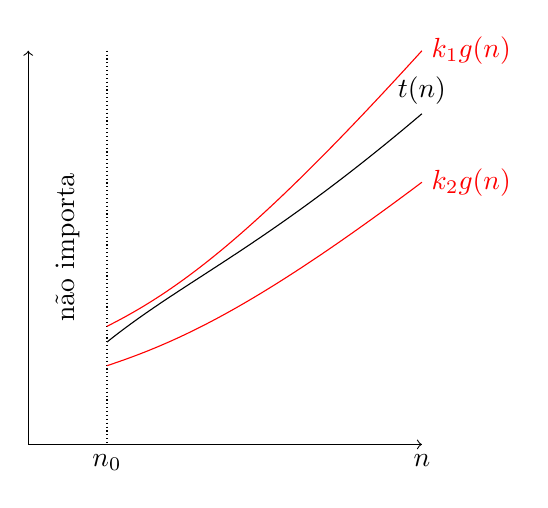
\begin{tikzpicture}
  \draw[->](0, 0) -- (5, 0)             node[below] {$n$};
  \draw[->](0, 0) -- (0, 5);
  \draw[densely dotted](1, 5) -- (1, 0) node[below] {$n_0$};
  \node[rotate=90] at (0.5, 2.5) {n\~{a}o importa};
  \draw[color=red] (1, 1.5) .. controls (2, 2) and (3, 2.8) .. (5, 5) node[above,right]{$k_1 g(n)$};
  \draw[color=red] (1, 1) .. controls (2, 1.33) and (3, 1.83) .. (5, 3.33) node[above,right]{$k_2 g(n)$};
  \draw (1, 1.3) .. controls (2, 2.1) and (3, 2.5) .. (5, 4.2) node[above]{$t(n)$};
\end{tikzpicture}